% !TeX encoding = utf-8
% !TeX program = xelatex
\documentclass[fntef]{ctexbeamer}
\usepackage{xunicode-addon}

\xeCJKsetup{
  AllowBreakBetweenPuncts=true,
  sout/thickness=.1em,
}

\usetheme{CambridgeUS}
\hypersetup{pdfpagemode=FullScreen}

\usepackage{multicol}

\usefonttheme{professionalfonts}
\usepackage{unicode-math}
\setmainfont{Cambria}
\setsansfont{Calibri}
\setmonofont{Consolas}
\setmathfont{Cambria Math}
\setCJKmainfont{Source Han Serif SC}[UprightFont={* Bold}]
\setCJKsansfont[BoldFont={* Bold}]{Source Han Sans SC}
\setCJKmonofont{Source Han Sans SC}
\newfontfamily\lmr{Latin Modern Roman}
\newfontfamily\lmss{Latin Modern Sans}
\newfontfamily\lmtt{Latin Modern Mono}
\renewfontfamily\useTIPAfont{Segoe UI}

\usepackage{mflogo}
\usepackage{metalogo}
\newcommand\BibTeX{{%
  \fontspec{TeX Gyre Heros}B\kern-.05em%
  \textsc{i\kern-.025em b}\kern-.08em%
  \TeX}}
\providecommand{\LyX}{L\kern-.1667em\lower.25em\hbox{Y}\kern-.125emX\@}

\usepackage{amsmath}
\usepackage{mathtools}


\usepackage{tikz}
\usetikzlibrary{positioning}
\usetikzlibrary{shapes.geometric}
\usetikzlibrary{shapes.symbols}
\usetikzlibrary{shapes.callouts}
\colorlet{shade}{blue!20}
\usepackage{pict2e}
\usepackage{animate}

\graphicspath{{figures/}}


\usepackage{booktabs}
\usepackage{makecell}
\newcolumntype{i}{!{\vrule width\lightrulewidth}}
\newcolumntype{I}{!{\vrule width\heavyrulewidth}}
\newcommand\Hline{\Xhline{\lightrulewidth}}
\newcommand\HLINE{\Xhline{\heavyrulewidth}}
\newcommand\Cline[1]{\Xcline{#1}{\lightrulewidth}}
\newcommand\CLINE[1]{\Xcline{#1}{\heavyrulewidth}}

\setbeamerfont{caption}{size=\footnotesize}

\usepackage{fancyvrb}
\fvset{formatcom=\usebeamercolor{structure}\color{fg!80!black}}
\AtBeginDocument{\DefineShortVerb{\|}}

\renewcommand\marginpar[2][]{}
\usepackage{democode}
\democodeset{
  font=\usebeamercolor{structure}\color{fg!80!black},
  backgroundcolor=white,
  widthfrac=0.55,
  outdir=tmp,
}
\def\thedemocode{\arabic{part}-\arabic{section}-\arabic{democode}}
\newcommand\textverb[1]{\texttt{#1}}

\newcommand\pkg[1]{\texttt{\usebeamercolor{structure}\color{fg!80!black}#1}}
\newsavebox\tmpbox

\usepackage{listings}

\usepackage{clrscode}

\usepackage{siunitx}
\usepackage{chemformula}


\usepackage{lettrine}
\usepackage{shapepar}

\setlength{\parskip}{.4\baselineskip plus .2\baselineskip minus .2\baselineskip}
% 在个别时候取消 \raggedright 的作用
\def\normalparagraph{\rightskip=0pt\spaceskip=0pt\xspaceskip=0pt\relax}

\setbeamercolor{quote}{bg=lightgray!50}
\setbeamerfont{quote}
    {family={\rmfamily},shape=\upshape,size=\footnotesize}

\newtheorem{thm}{定理}[section]

% fix ctex-kit issue #489
\ExplSyntaxOn
\makeatletter
\cs_set_protected_nopar:Npn \CTEX@disableautoindent
  { \tl_clear:N \l__ctex_autoindent_tl }
\makeatletter
\ExplSyntaxOff

\AtBeginPart{\frame{\partpage}}
\AtBeginSection{
  \begin{frame}{内容}
    \tableofcontents[currentsection,hideallsubsections]
  \end{frame}
}
\AtBeginSubsection{
  \begin{frame}{内容}
    \tableofcontents[currentsection,subsectionstyle=show/shaded/hide]
  \end{frame}
}

\title{多元分析方法使用报告}
\author{刘士坤\quad 郑辉杨\quad 薛兆浩\quad 余涛}
\institute[]{天津商业大学\quad 统计系}
\date{2020 年 10 月 21 日}
\subject{多元分析}
\keywords{聚类分析 线性判别分析 主成分分析}
\hypersetup{pdftitle=多元分析方法使用报告,pdfauthor=刘士坤}


\setbeamertemplate{itemize items}{\color{black}$\bullet$}
\setbeamertemplate{sections/subsections in toc}[circle]
\usepackage{float}
\usepackage{xkeyval}

\begin{document}

% !TeX root = multianalysis.tex
% !TeX encoding = UTF-8
% !TeX program = XeLaTeX

\begin{frame}

\begin{tikzpicture}[overlay]
\pgfmathdeclarerandomlist{symbols}{%
  {\texttt{\string Cluster}}%
  {\texttt{\string LDA}}
  {\texttt{\string PCA}}
  {\texttt{\string Factor}}}
\foreach \y in {0,-1,...,-7} {
  \foreach \x in {0,1,...,12} {
    \pgfmathrandomitem{\randsymbol}{symbols}
    \node[black!15,rotate=45] at (\x,\y) {\randsymbol};
  }
}
\end{tikzpicture}
\titlepage
\end{frame}

\begin{frame}{本次报告所使用的分析方法}
  % \pause
    \begin{itemize}%%[<+->]
        \item 聚类分析(Cluster analysis)
        \begin{itemize}
          \item 系统聚类(Hierarchical clustering)
          \item K-means聚类(k-means clustering)
        \end{itemize}

        \item 主成分分析(Principal component analysis)

        \item 线性判别分析(Linear discriminant analysis)
        % \begin{itemize}
        %   \item Fisher 线性判别(Fisher's linear discriminant)
        %   \item Bayes 判别(Bayes discriminant)
        % \end{itemize}
    \end{itemize}
\strut
\end{frame}

\begin{frame}{本次报告所使用的数据}{某中学火箭班、实验班、重点班、普通班80名同学的期中考试成绩}
  \begin{columns}
    \column{.5\textwidth}
    \begin{figure}
      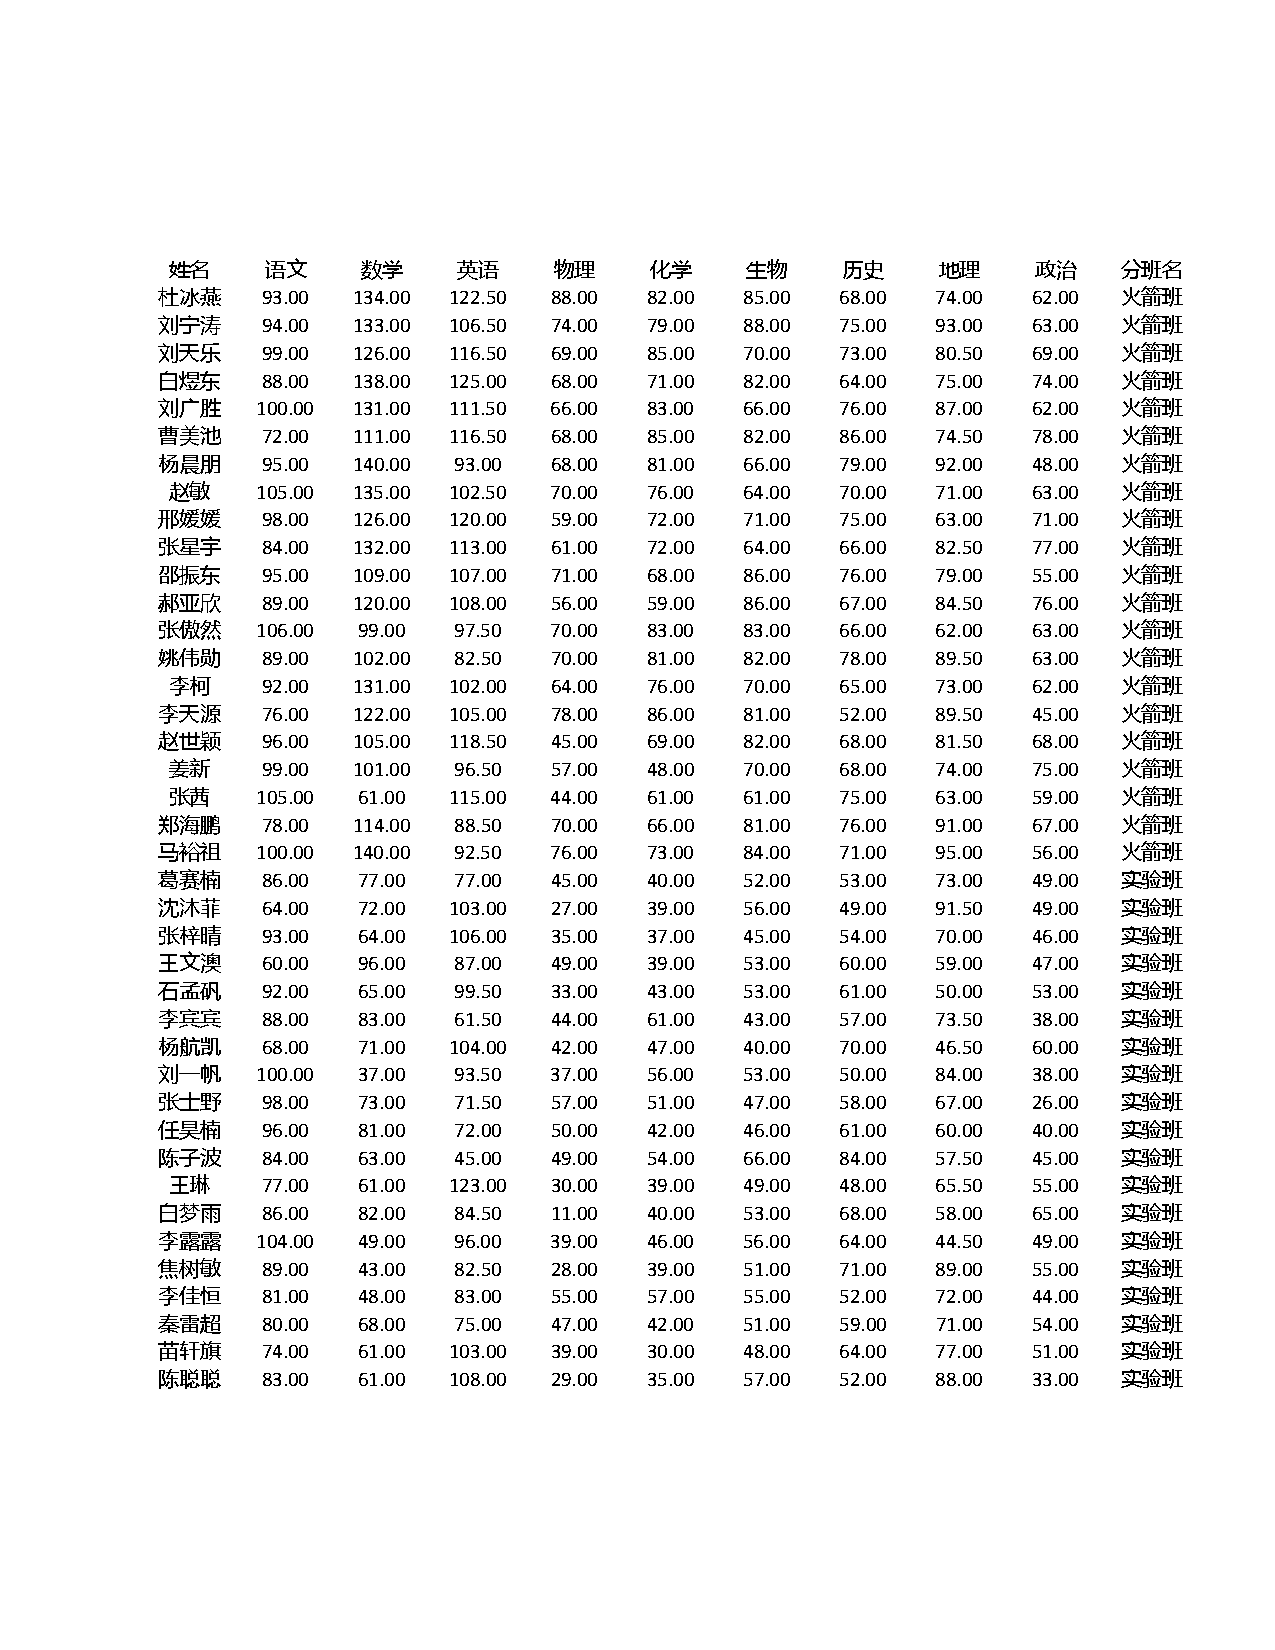
\includegraphics[height=7.7cm]{grades1.pdf}
    \end{figure}

    \column{.5\textwidth}
    \begin{figure}
      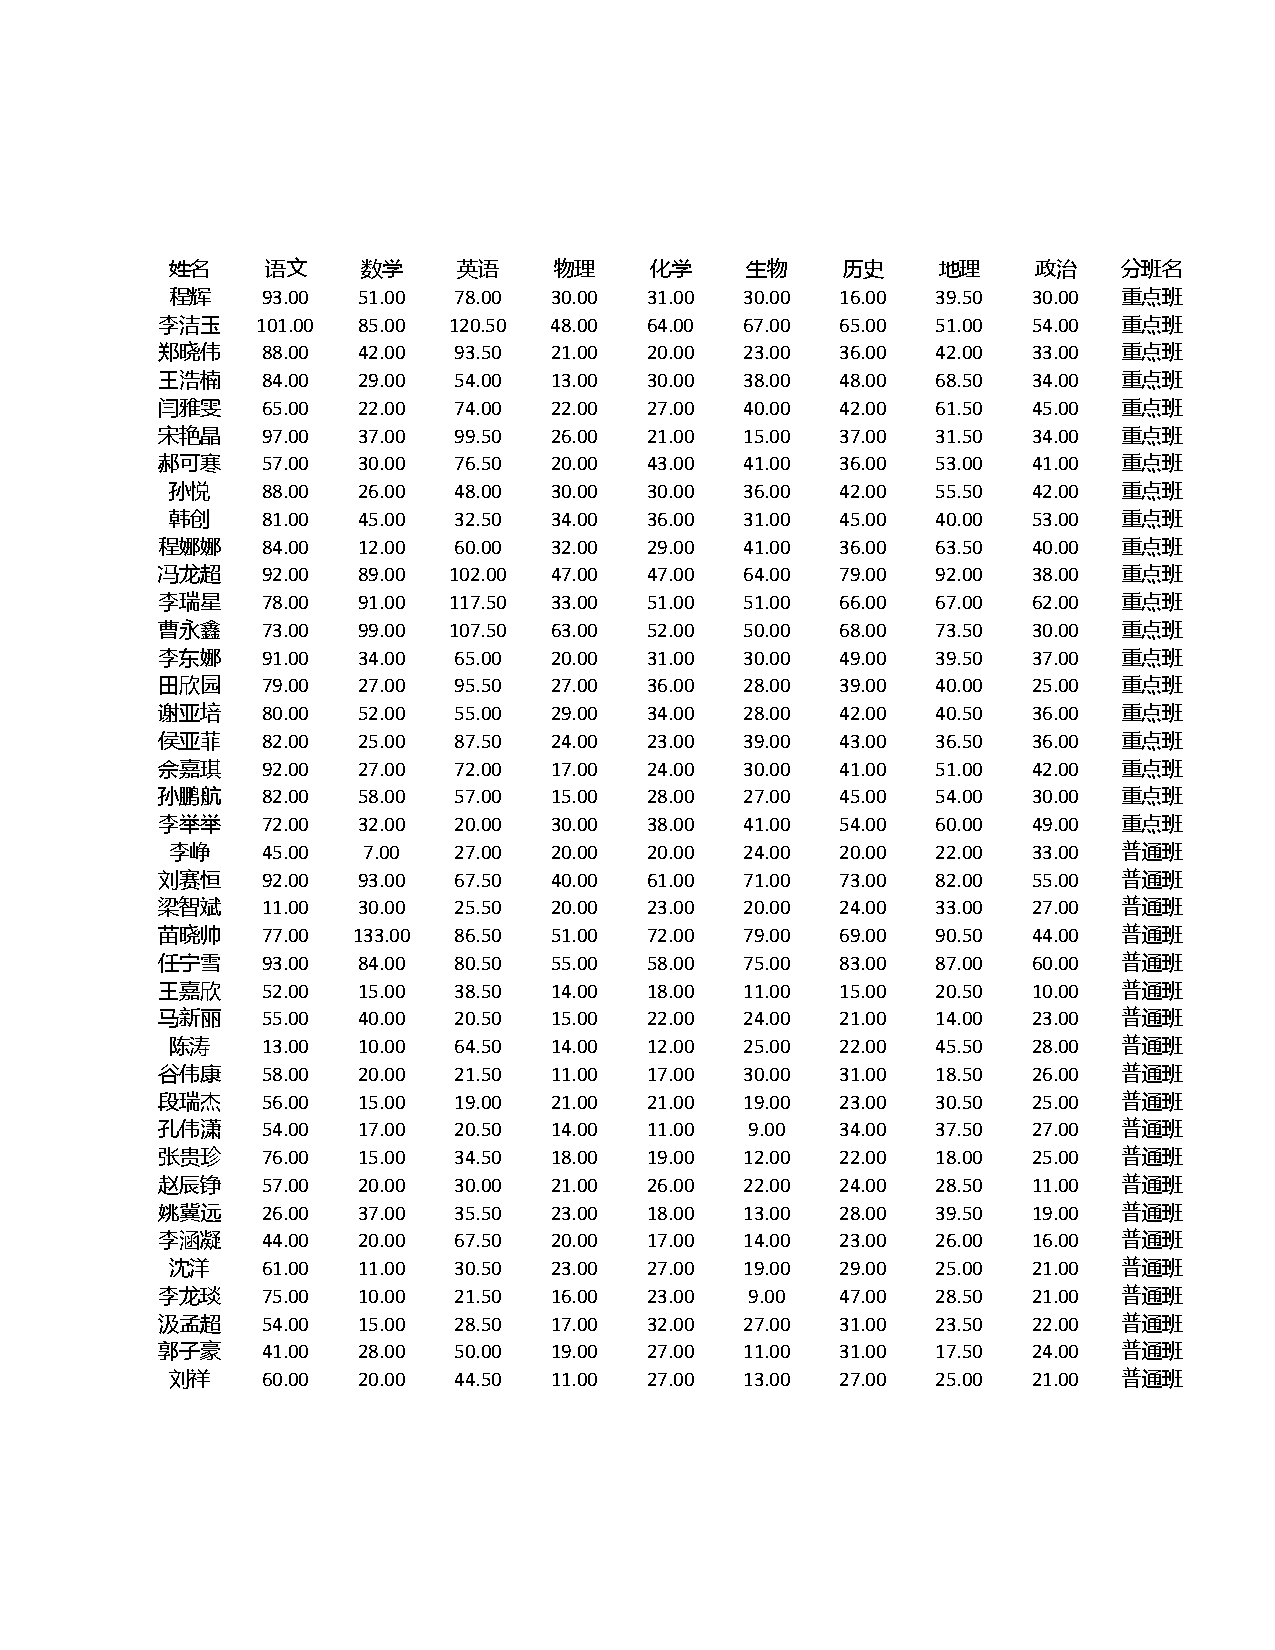
\includegraphics[height=7.7cm]{grades2.pdf}
    \end{figure}
  \end{columns}
  \strut
\end{frame}


% !TeX root = multianalysis.tex
% !TeX encoding = UTF-8
% !TeX program = XeLaTeX


\part{聚类分析(Cluster analysis)}

\section{描述性统计}

\begin{frame}{描述性统计}
    \begin{center}
        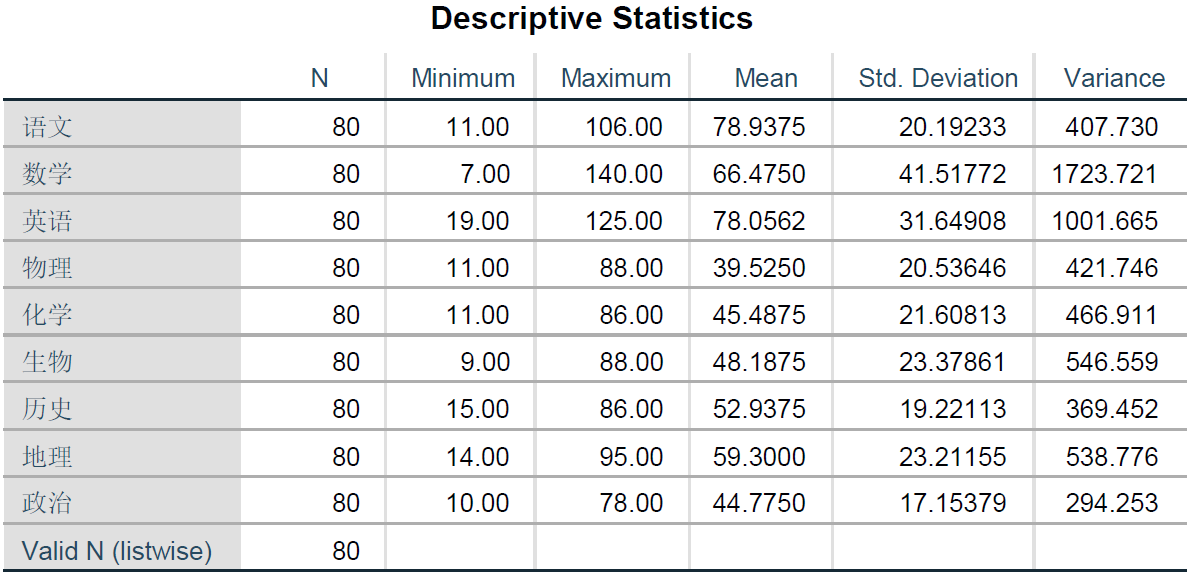
\includegraphics[scale=0.285]{descriptive.png}
    \end{center}
    \vspace{-0.5cm}
\end{frame}

\section{对指标变量(9个学科)进行系统聚类}

\begin{frame}{选择平方欧氏距离时的距离矩阵}
    \begin{center}
        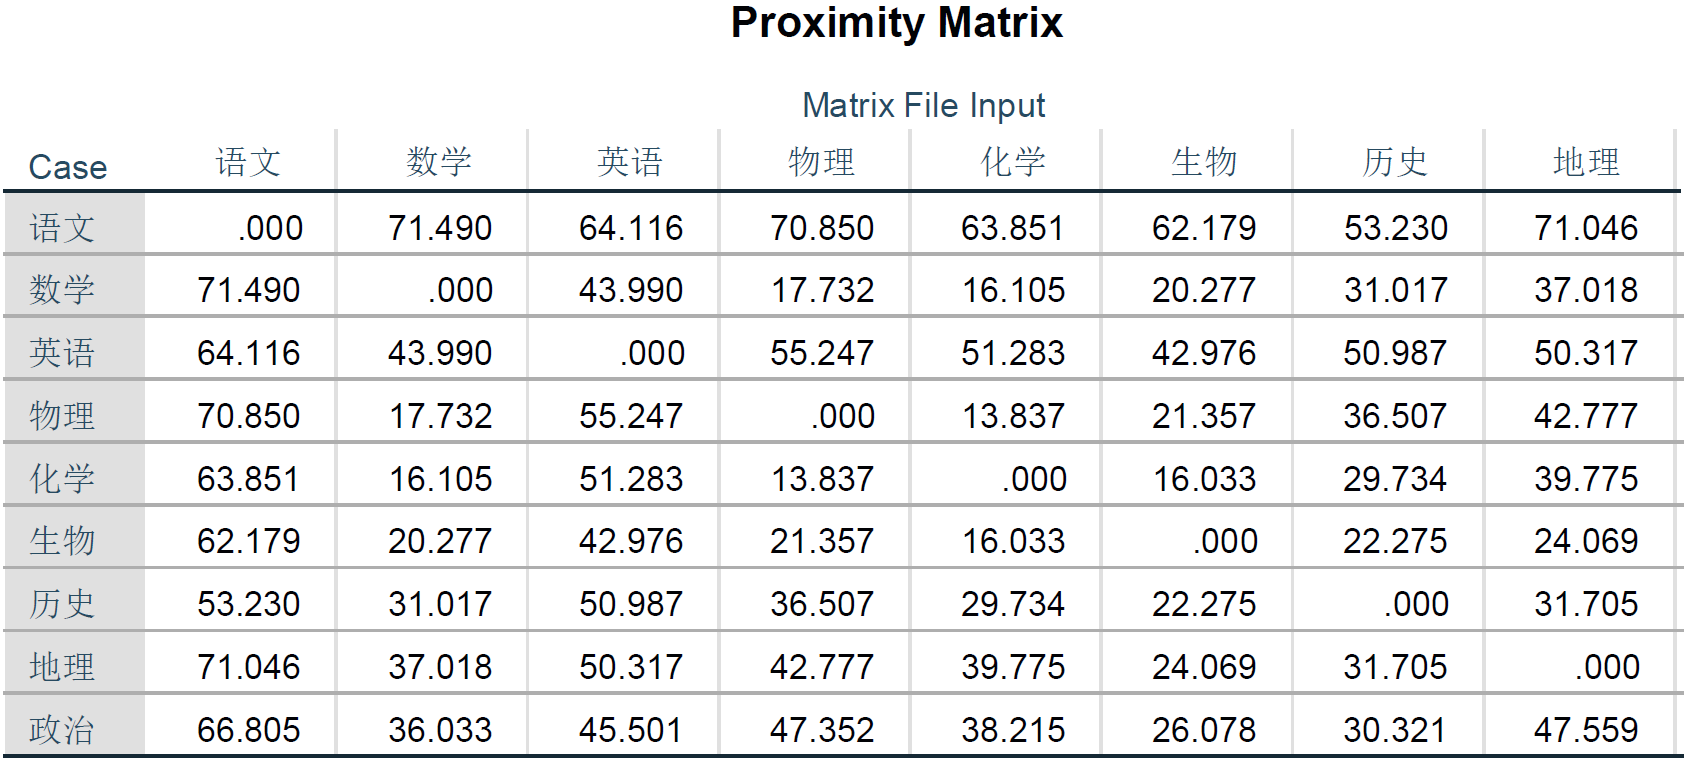
\includegraphics[scale=0.2]{平方欧氏距离距离矩阵.png}
    \end{center}
    \vspace{-0.5cm}
\end{frame}

\begin{frame}{组内联结法的谱系聚类图}
    \begin{center}
        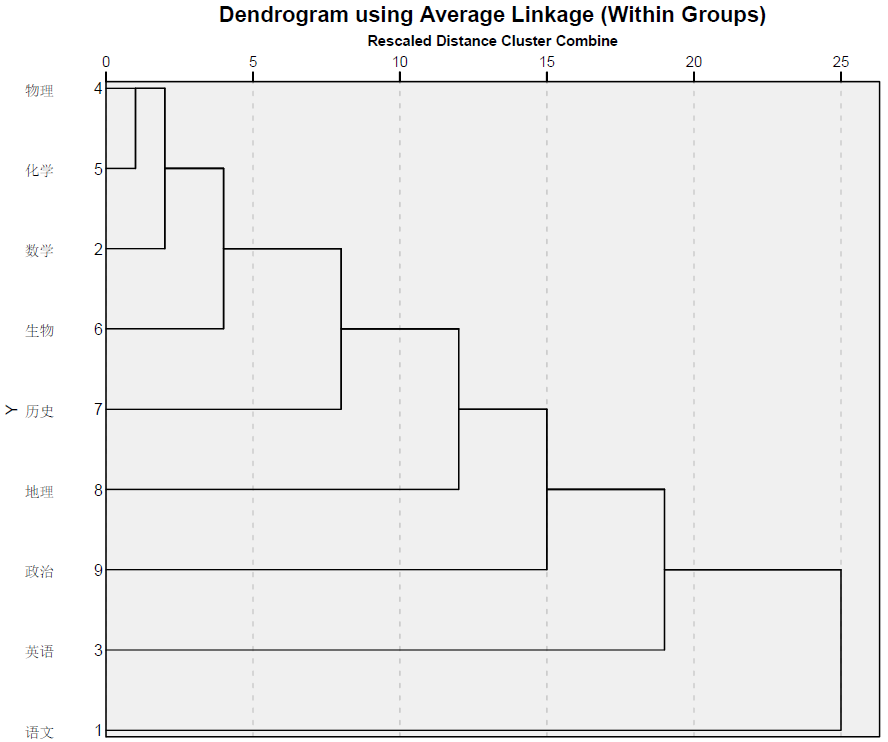
\includegraphics[scale=0.25]{组内联结法谱系聚类图.png}
    \end{center}
    \vspace{-0.5cm}
\end{frame}


\begin{frame}{选择聚成4类的结果}
    \begin{center}
        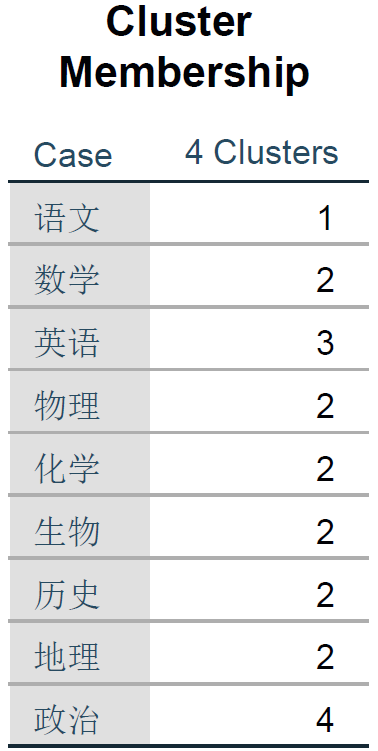
\includegraphics[scale=0.25]{聚类结果.png}
    \end{center}
    \vspace{-0.5cm}
\end{frame}


\section{对样品(80名同学)进行 K-means 聚类}

\begin{frame}{4个初始中心}
    \begin{center}
        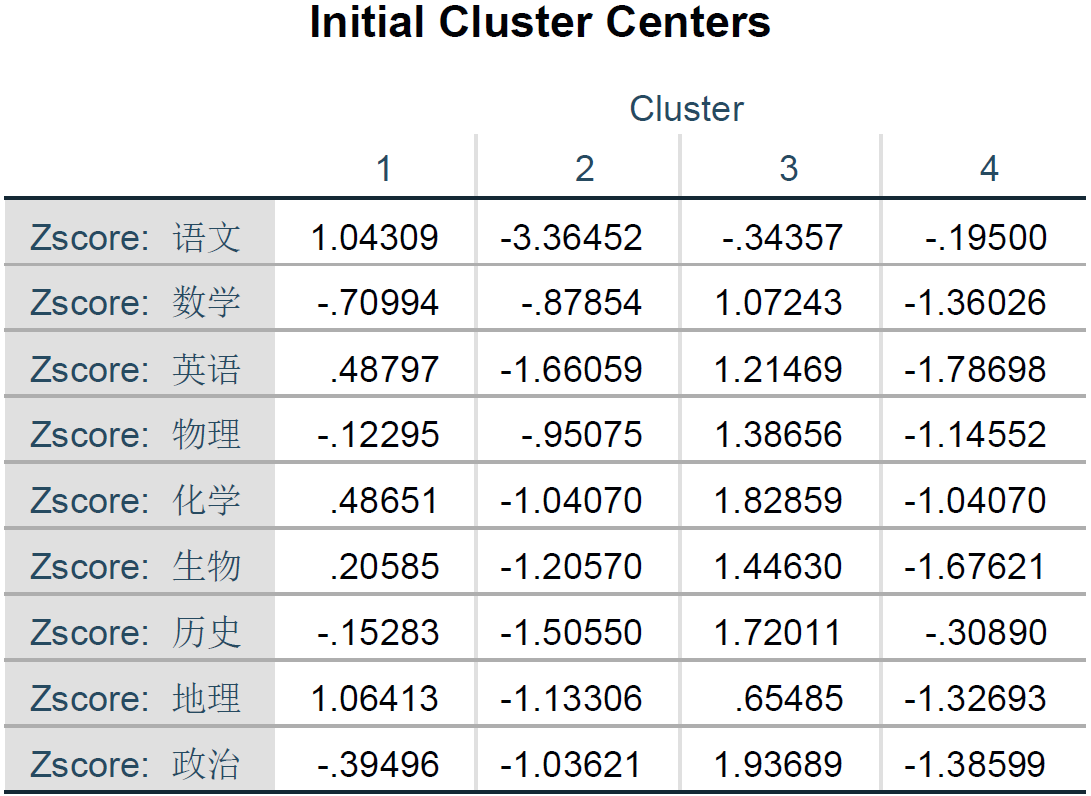
\includegraphics[scale=0.235]{4个初始中心.png}
    \end{center}
    \vspace{-0.5cm}
\end{frame}

\begin{frame}{聚类结果}
    \begin{figure}[H]
        \centering
        \begin{minipage}{0.32\textwidth}
            \centering
            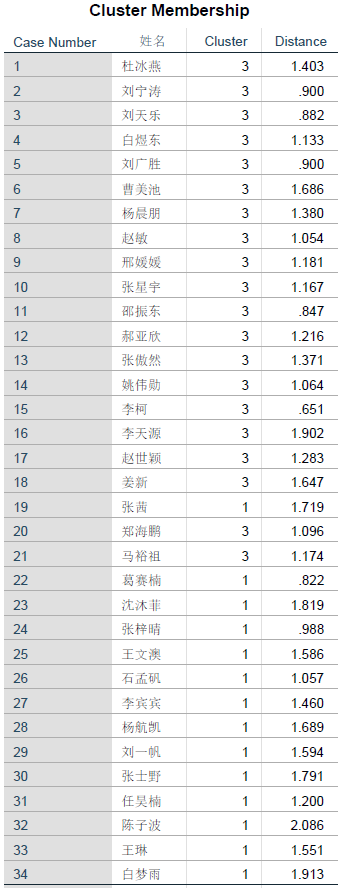
\includegraphics[scale=0.23]{聚类结果1.png}
        \end{minipage}
        \begin{minipage}{0.32\textwidth}
            \centering
            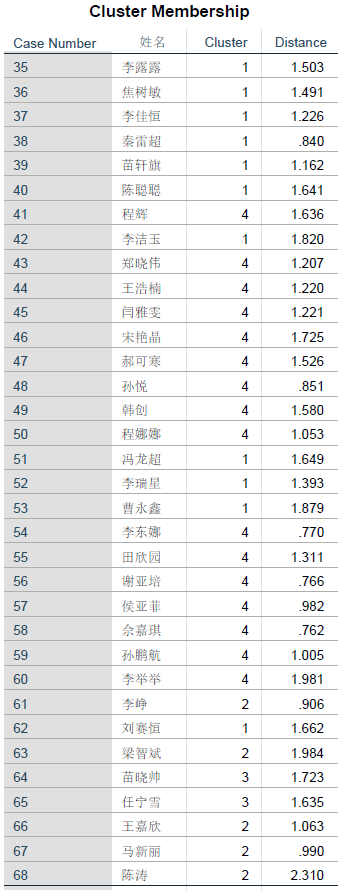
\includegraphics[scale=0.23]{聚类结果2.png}
        \end{minipage}
        \begin{minipage}{0.32\textwidth}
            \centering
            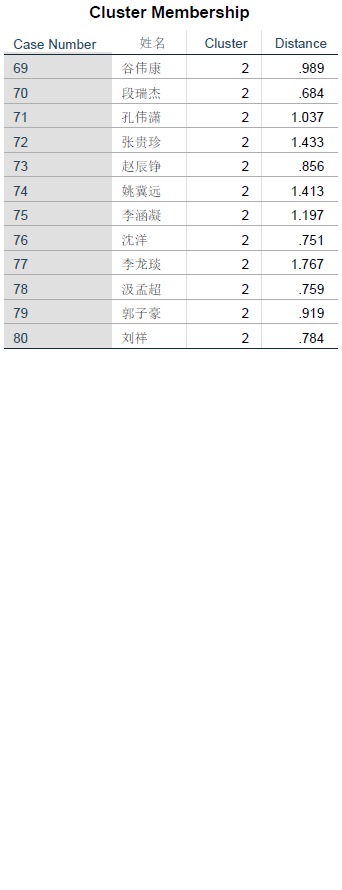
\includegraphics[scale=0.23]{聚类结果3.png}
        \end{minipage}
    \end{figure}
\end{frame}

\begin{frame}{各类中的样品数}
    \begin{center}
        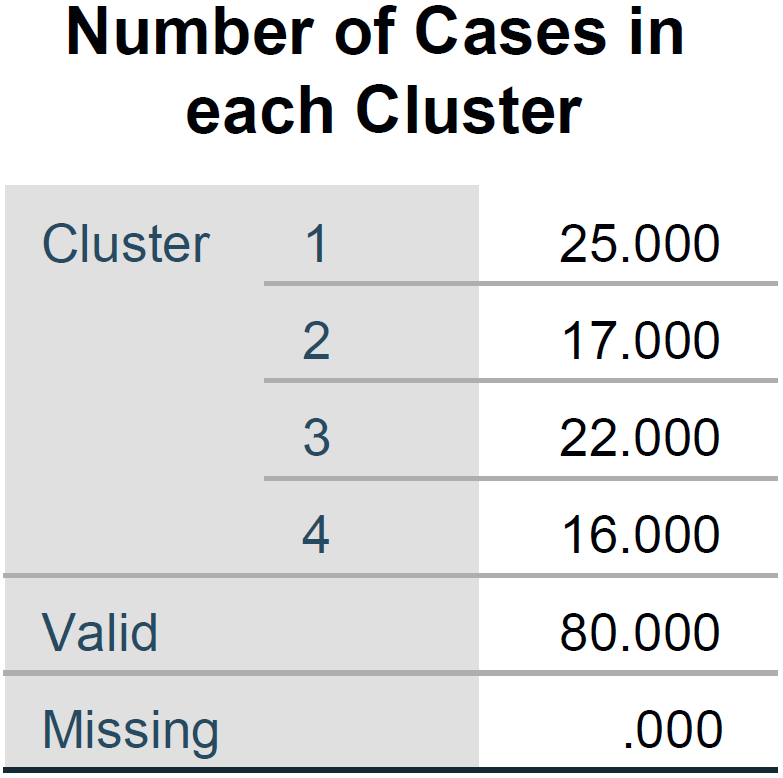
\includegraphics[scale=0.2]{各类的样品数.png}
    \end{center}
    \vspace{-0.5cm}
\end{frame}


\begin{frame}{方差分析表}
    \begin{center}
        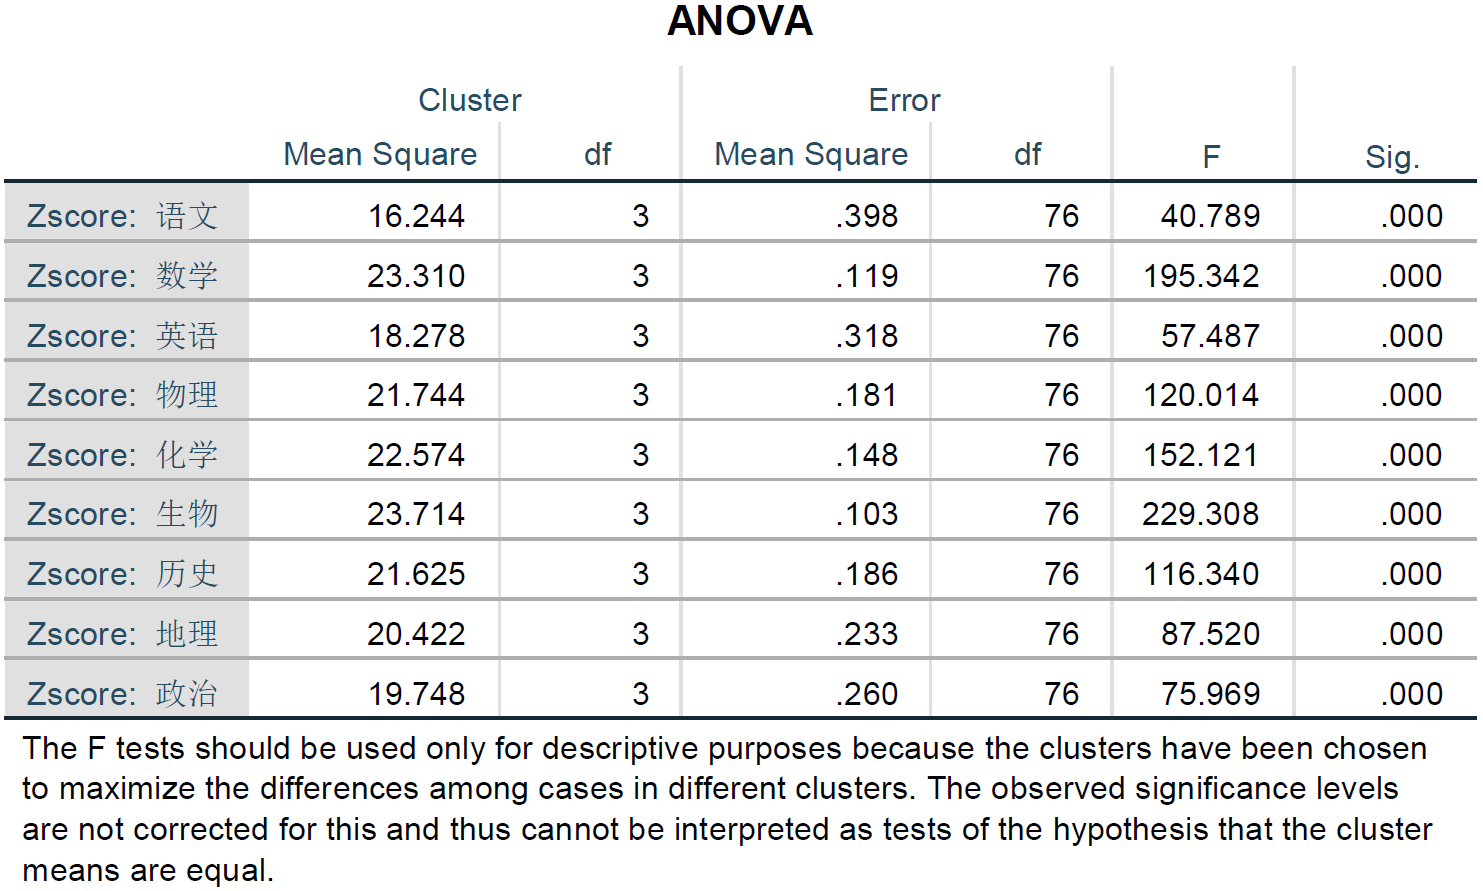
\includegraphics[scale=0.215]{方差分析表.png}
    \end{center}
    \vspace{-0.5cm}
\end{frame}


% !TeX root = multianalysis.tex
% !TeX encoding = UTF-8
% !TeX program = XeLaTeX

\part{主成分分析\\(Principal component analysis)}


\begin{frame}{样本相关阵}
    \begin{center}
        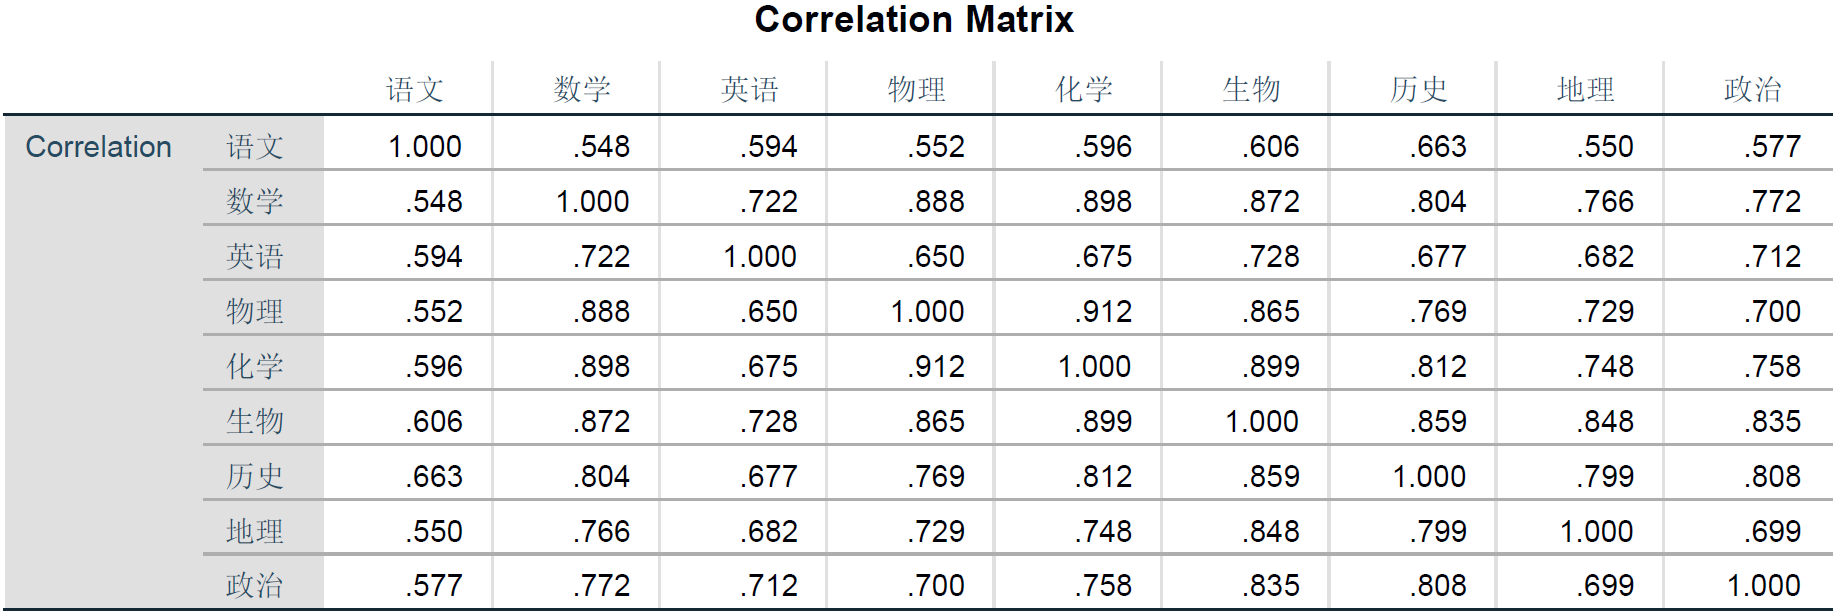
\includegraphics[scale=0.185]{样本相关阵.png}
    \end{center}
    \vspace{-0.5cm}
\end{frame}


\begin{frame}{公因子方差表}
    \begin{center}
        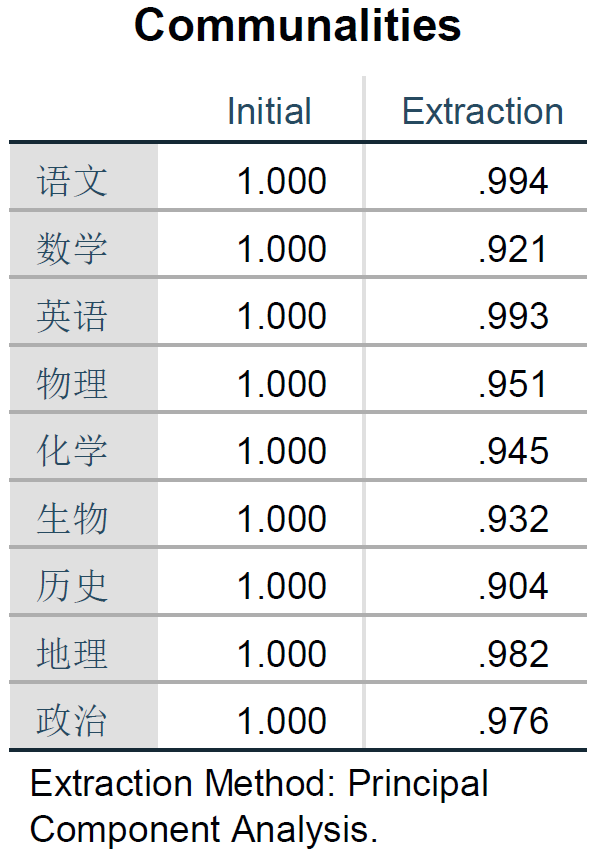
\includegraphics[scale=0.36]{公因子方差表.png}
    \end{center}
    \vspace{-0.5cm}
\end{frame}


\begin{frame}{各个主成分解释原始变量总方差表}
    \begin{center}
        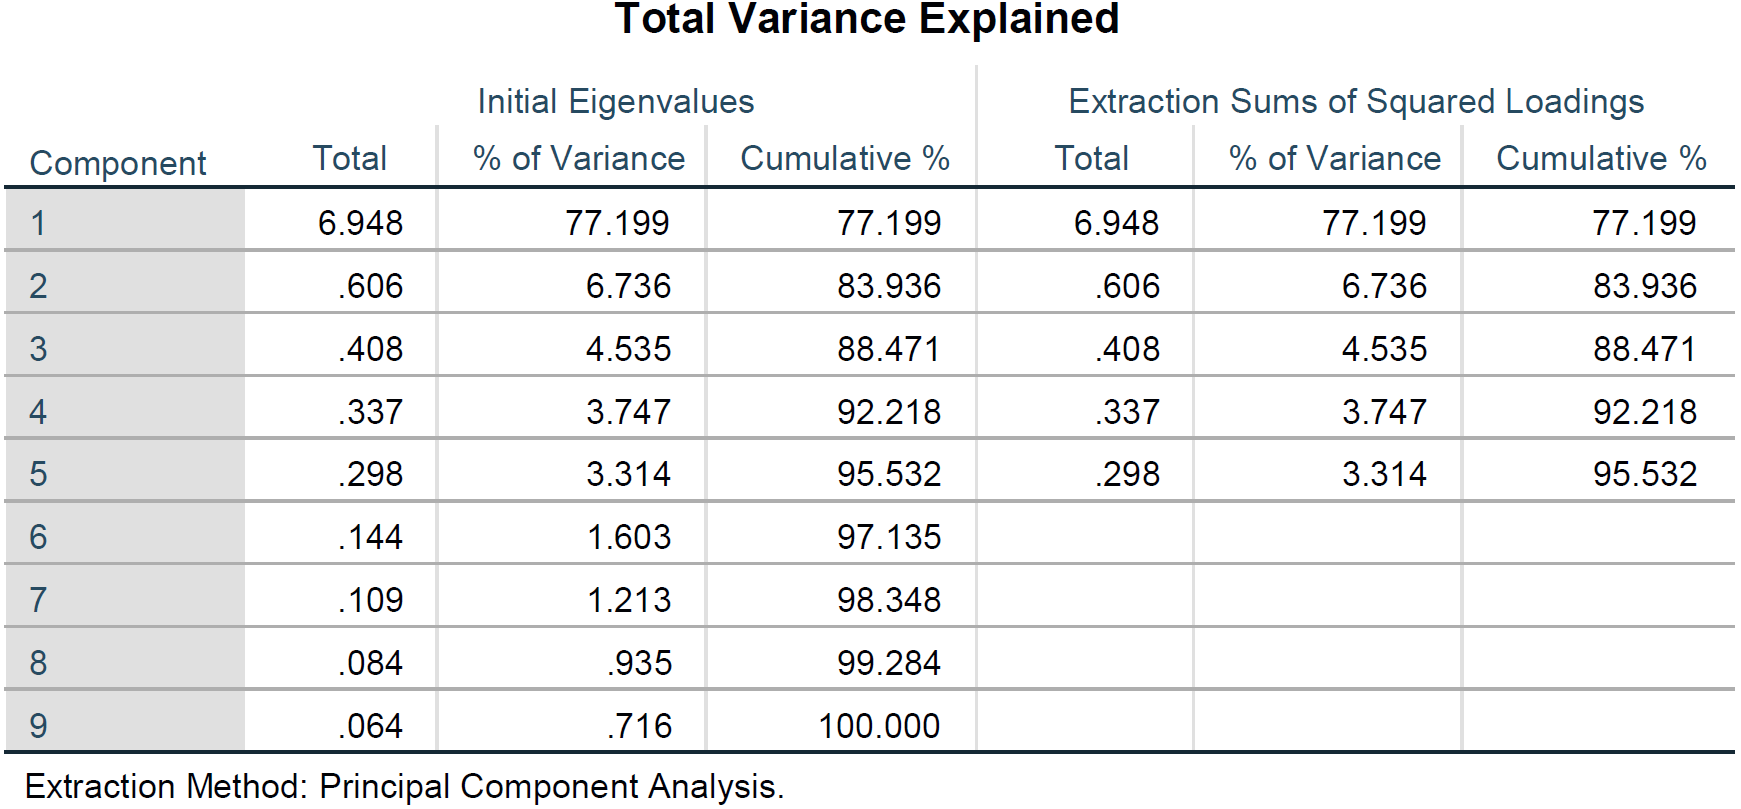
\includegraphics[scale=0.195]{总方差解释表.png}
    \end{center}
    \vspace{-0.5cm}
\end{frame}


\begin{frame}{成分矩阵}
    \begin{center}
        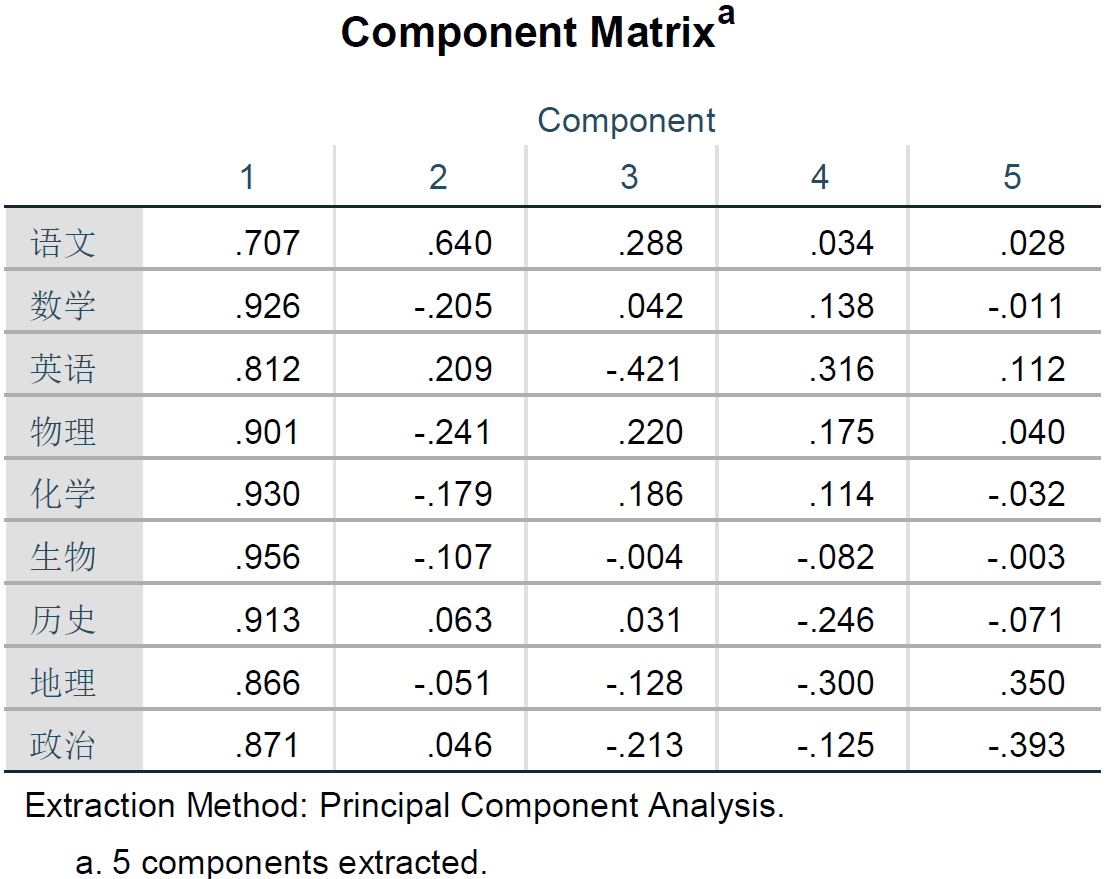
\includegraphics[scale=0.21]{成分矩阵.png}
    \end{center}
    \vspace{-0.5cm}
\end{frame}


\begin{frame}

    \footnotesize
    \begin{align*}
        y_1 &= 0.268x_1+0.351x_2+0.308x_3+0.342x_4+ 0.353x_5+0.363x_6+ 0.346x_7+\\
           &\quad \ \begin{multlined}[t]
            0.329x_8+0.330x_9
           \end{multlined}
    \end{align*}
    
    \begin{align*}
        y_2&=0.822x_1 -0.263x_2 + 0.268x_3 -0.310x_4 -0.230x_5 -0.137x_6 + 0.081x_7 - \\
        & \quad \ \begin{multlined}[t]
            0.066x_8 + 0.059x_9
        \end{multlined}
    \end{align*}

    \begin{align*}
        y_3 &=0.451x_1 + 0.066x_2 -0.659x_3 + 0.344x_4+  0.291x_5 -0.006x_6 + 0.049x_7 - \\
        &\quad \ \begin{multlined}[t]
            0.200x_8 -0.333x_9
        \end{multlined}
    \end{align*}

    \begin{align*}
        y_4 &= 0.059x_1 + 0.238x_2 + 0.544x_3 + 0.301x_4 + 0.196x_5 -0.141x_6 -0.424x_7 - \\
        &\quad \ \begin{multlined}[t]
            0.518x_8 -0.215x_9
        \end{multlined}
    \end{align*}

    \begin{align*}
        y_5 &= 0.051x_1 -0.020x_2 + 0.205x_3 + 0.073x_4 -0.059x_5 -0.005x_6 -0.130x_7 + \\
        & \quad \ \begin{multlined}[t]
            0.641x_8 -0.720x_9
        \end{multlined}
    \end{align*}

\end{frame}



% !TeX root = multianalysis.tex
% !TeX encoding = UTF-8
% !TeX program = XeLaTeX


\part{线性判别分析\\(Linear discriminant analysis)}


\begin{frame}{对主成分均值的检验}
    \begin{center}
        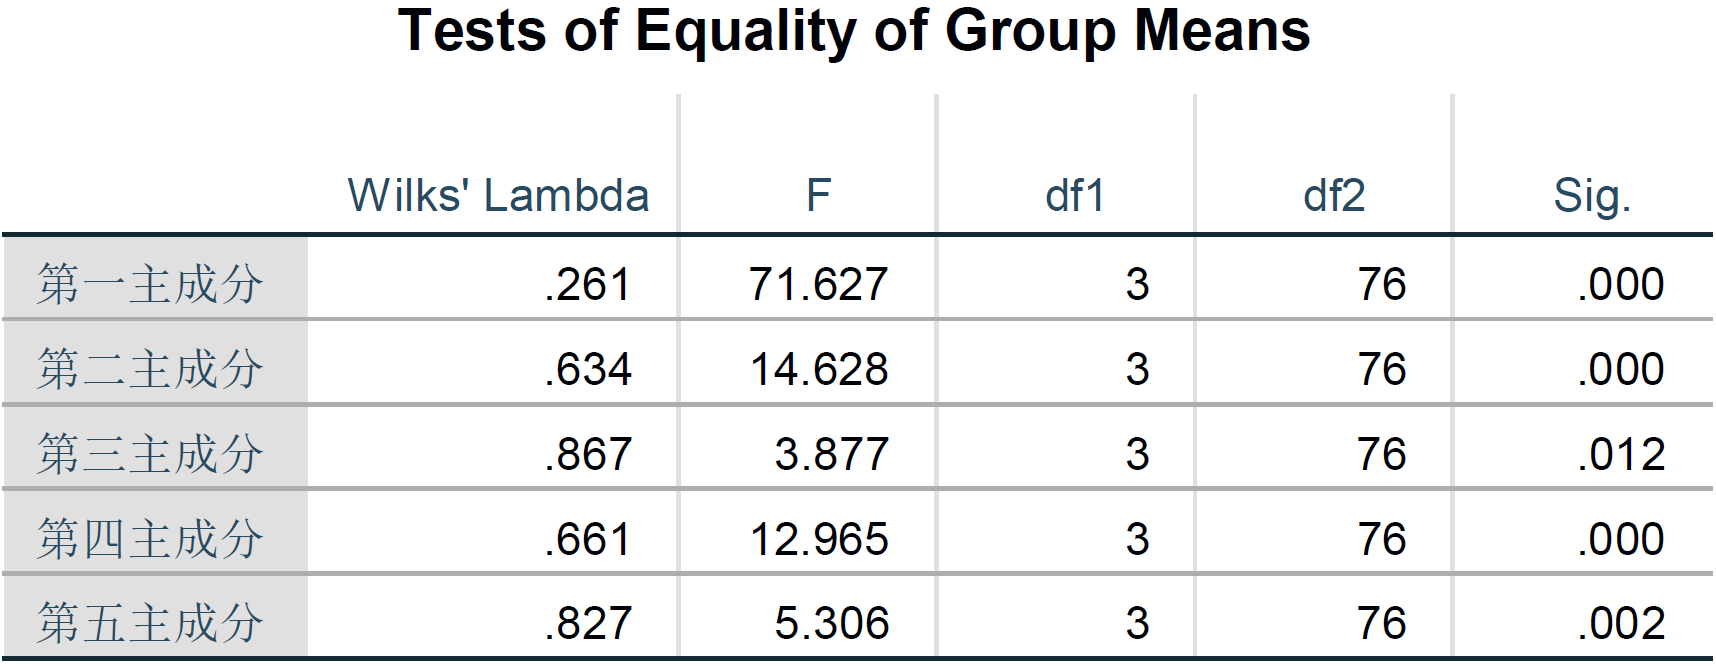
\includegraphics[scale=0.2]{主成分的均值检验.png}
    \end{center}
    \vspace{-0.5cm}
\end{frame}


\begin{frame}{对主成分协方差矩阵的 Box's M 检验}
    \begin{center}
        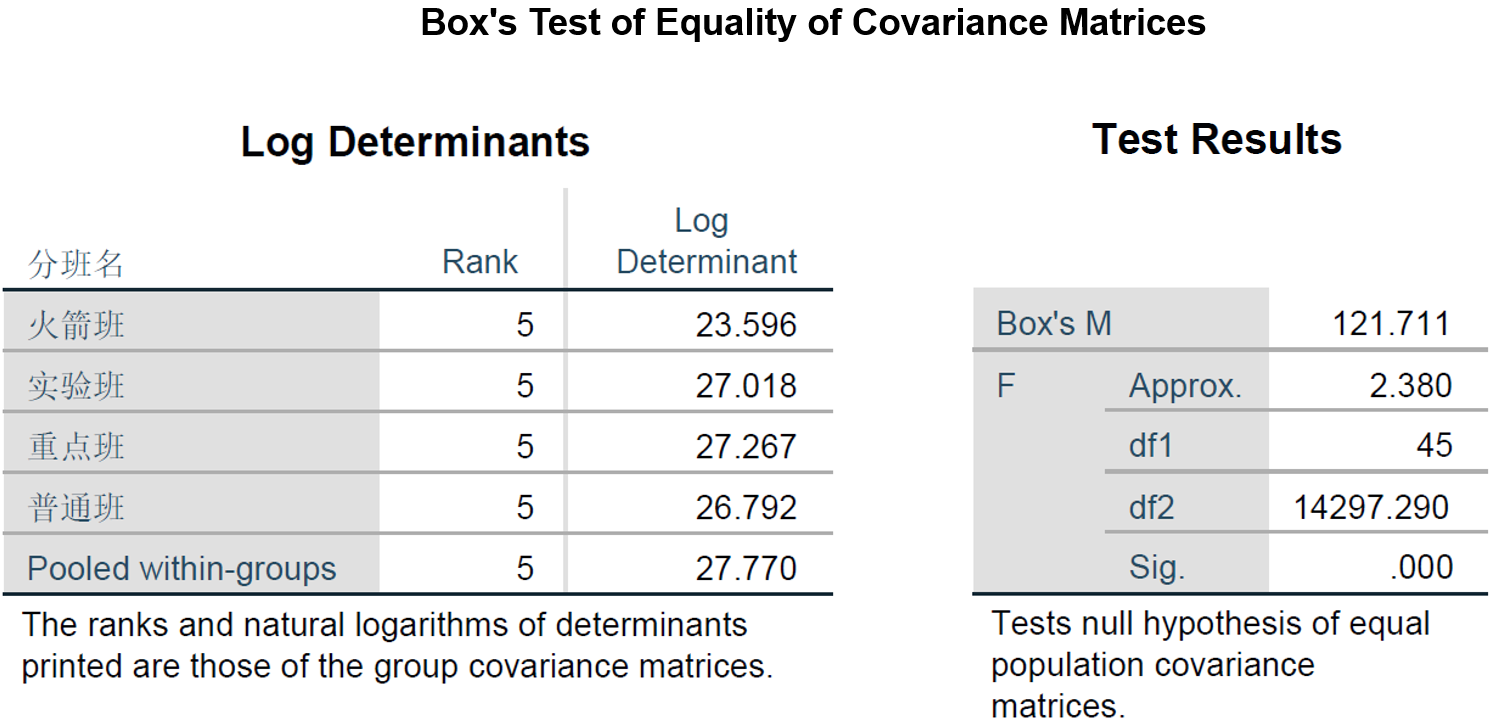
\includegraphics[scale=0.22]{协方差阵相等的检验.png}
    \end{center}
    \vspace{-0.5cm}
\end{frame}


\begin{frame}{Fisher 线性判别}
    \begin{center}
        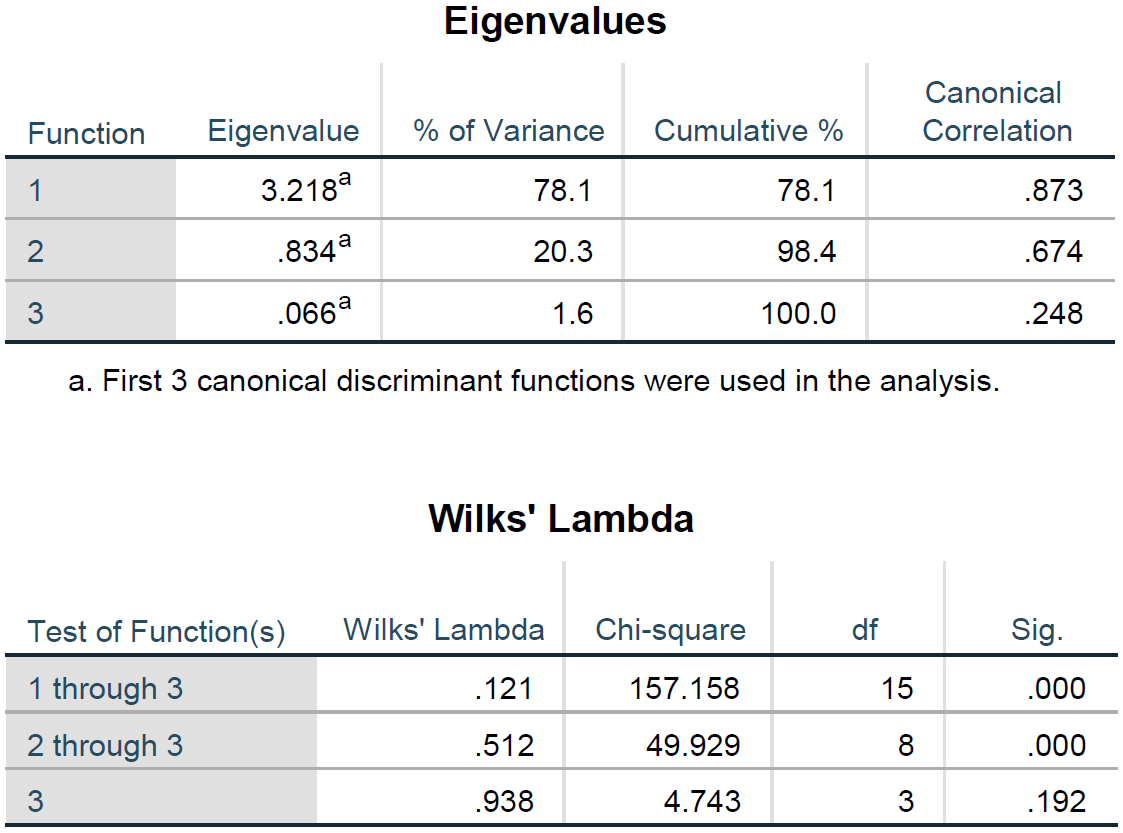
\includegraphics[scale=0.225]{判别函数特征根、解释方差比.png}
    \end{center}
    \vspace{-0.5cm}
\end{frame}


\begin{frame}{标准化/非标准化 Fisher 线性判别函数}

    \begin{center}
        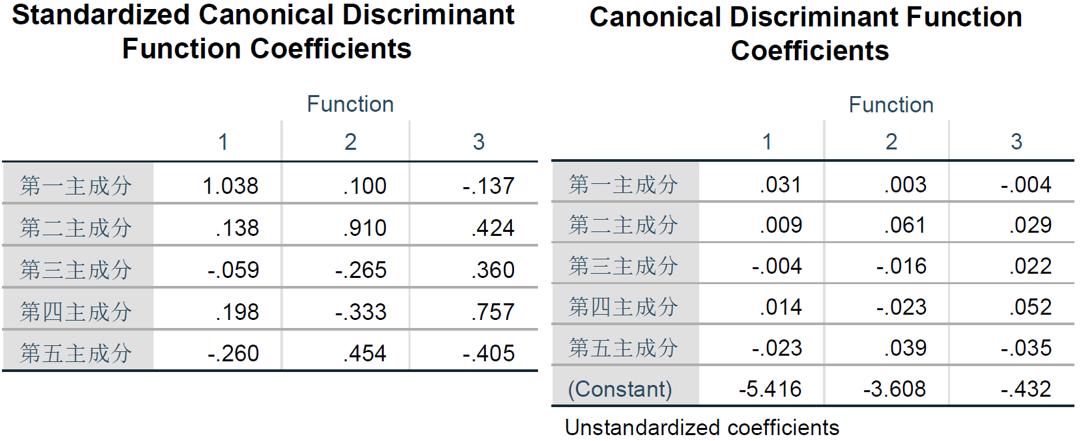
\includegraphics[scale=0.32]{标准化、非标准化判别系数.png}
    \end{center}
    \vspace{-0.5cm}

\end{frame}


% 分类函数.png
\begin{frame}{分类函数}
    \begin{center}
        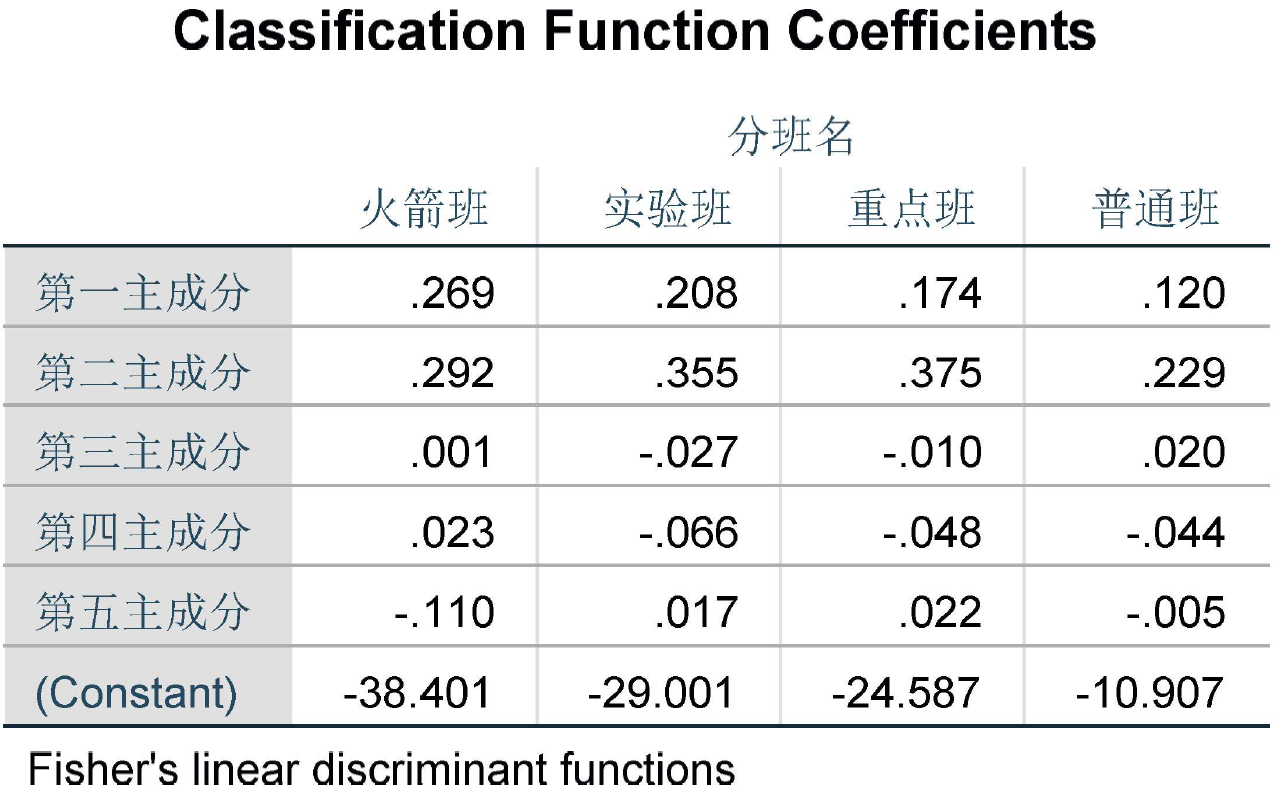
\includegraphics[scale=0.22]{分类函数.png}
    \end{center}
    \vspace{-0.5cm}
\end{frame}


% 分类结果.png
\begin{frame}{预测的分类结果}
    \begin{center}
        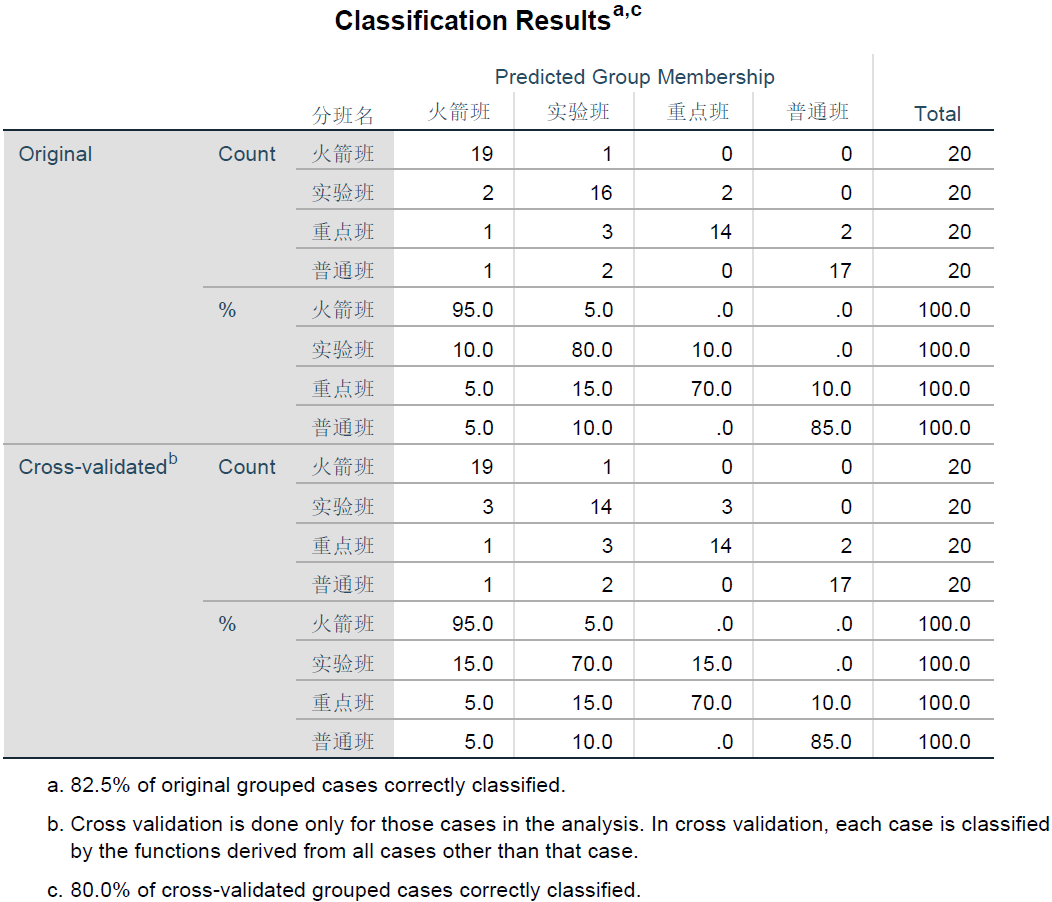
\includegraphics[scale=0.21]{分类结果.png}
    \end{center}
    \vspace{-0.5cm}
\end{frame}


% 分类结果图.png
\begin{frame}{预测的分类结果图}
    \begin{center}
        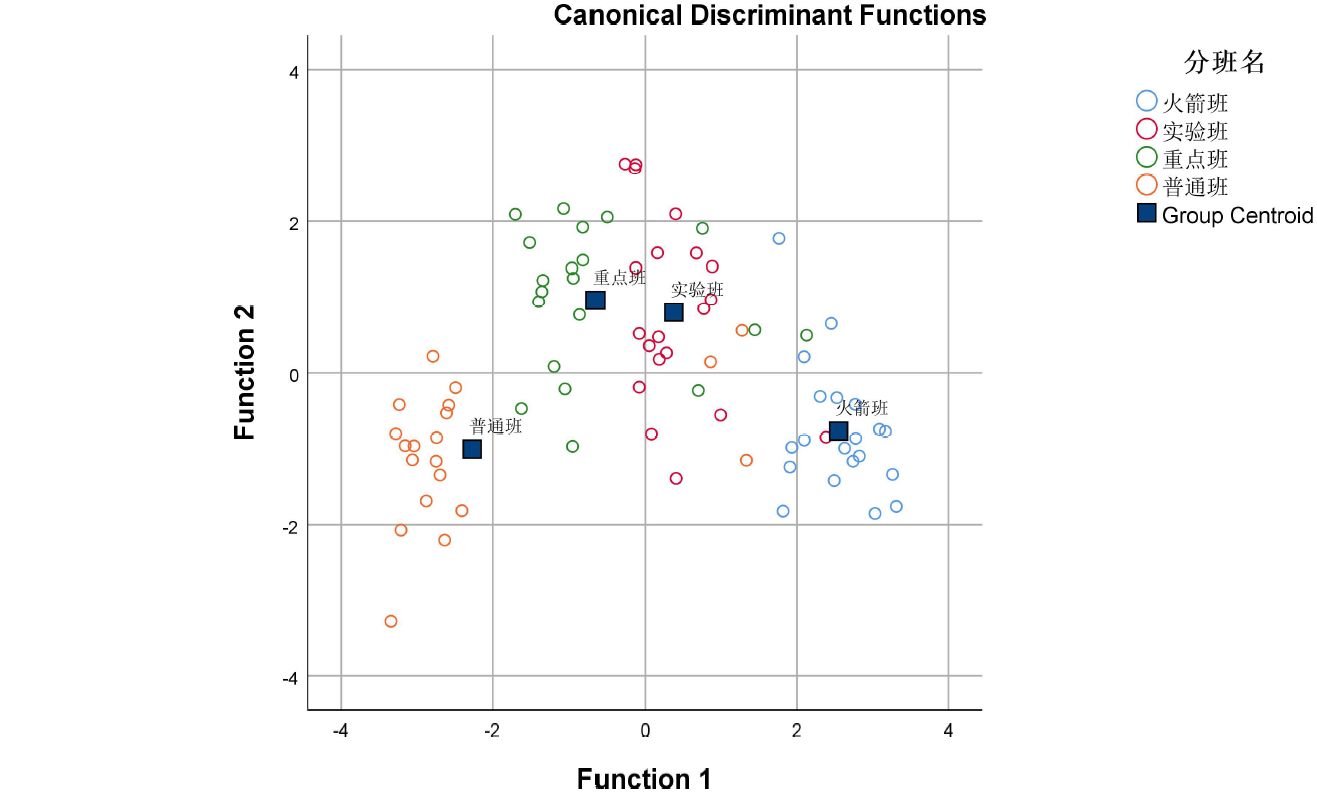
\includegraphics[scale=0.23]{分类结果图.png}
    \end{center}
    \vspace{-0.5cm}
\end{frame}


% !TeX root = multianalysis.tex
% !TeX encoding = UTF-8
% !TeX program = XeLaTeX


\begin{frame}[fragile]
    \frametitle{参考文献}
    % \begin{multicols}{1}
    \tiny
    \begin{thebibliography}{99}
        \bibitem{}
        \textsc{何晓群}.
        \newblock 多元统计分析 [M]. 2019.
        \newblock 北京: 中国人民大学出版社

        \bibitem{}
        \textsc{白志东}.
        \newblock 大维统计分析 [M]. 2012.
        \newblock 北京:高等教育出版社

        % \bibitem{}
        % \textsc{陈希孺}.
        % \newblock 数理统计学教程 [M]. 2009.
        % \newblock 合肥:中国科学技术大学出版社

        % \bibitem{}
        % \textsc{陈希孺}.
        % \newblock 数理统计学简史 [M]. 2002.
        % \newblock 长沙:湖南教育出版社

        \bibitem{}
        \textsc{Vincent Spruyt}.
        \newblock A geometric interpretation of the covariance matrix [EB/OL]. 2014.
        \newblock Computer vision for dummies
        \newblock \url{https://www.visiondummy.com/2014/04/geometric-interpretation-covariance-matrix}
        
        \end{thebibliography}
    % \end{multicols}
\end{frame}


\begin{frame}
    
\begin{tikzpicture}[overlay]
    \pgfmathdeclarerandomlist{symbols}{%
      {\texttt{\string Cluster}}%
      {\texttt{\string LDA}}
      {\texttt{\string PCA}}
      {\texttt{\string Factor}}}
    \foreach \y in {0,-1,...,-7} {
      \foreach \x in {0,1,...,12} {
        \pgfmathrandomitem{\randsymbol}{symbols}
        \node[black!15,rotate=45] at (\x,\y) {\randsymbol};
      }
    }
    \end{tikzpicture}
    \titlepage
\end{frame}

\end{document}
